% !TEX root = ../MasterThesis_goto_v1.tex

%%%%%%%%%%%%%%%%%%%%%%%%%%%%%%%%%%%%%%%%%%%%%%%%%%%%%%%%%%%%%%%%%%%%%%%%%%%%%%%%%%%%%%%%%%%%%%%%%%%%%
\chapter{現行の手法との比較} \label{chap:Comparison}

本研究での崩壊点検出の性能の可否についての判断は現行の手法と比較することによって行う。
本章では, そのような比較について議論を行う。
まず\ref{Com:ComparisonwithVF}節では崩壊点検出単体での性能を比較する。

崩壊点検出はジェットの再構成における最初段のアルゴリズムである。
したがって, 最終的な物理解析への影響や性能を確認するには, 本研究で作成した崩壊点検出を用いたフレーバータギングの性能を評価する必要がある。
このようなフレーバータギングの性能を確認する為, 本研究で作成した崩壊点検出アルゴリズムをLCFIPlus, Marlinで動作可能な形で実装した。
\ref{Com:FlavorTaggingComparison}節ではフレーバータギングを用いたより詳細な比較について述べる。


%%%%%%%%%%%%%%%%%%%%%%%%%%%%%%%%%%%%%%%%%%%%%%%%%%%%%%%%%%%%%%%%%%%%%%%%%%%%%%%%%%%%%%%%%%%%%%%%%%%%%
\section{崩壊点検出単体での比較} \label{Com:ComparisonwithVF}

本研究における崩壊点検出の性能を表\ref{PerformanceofAllEvents}に示した。
表\ref{PerformanceofLCFIPlus}にLCFIPlusで使用されている崩壊点検出の性能である文献\cite{LCFIPlusPaper}の値を示す。
これは本研究の目標値である。
\ref{VFDL:TPVFDL:VertexProduction}項でも述べたように, この評価項目はPrimaryやOthersについては低ければ, BottomやCharmについては高ければ良い性能であるとみなせる。
崩壊点検出での比較では, BottomやCharmの再構成効率が$10\%$以上向上しているとわかる。
一方で, $0.5$より高い閾値を「任意の数の飛跡についてのネットワーク」の出力に設け, より純度の高いsecondary vertexの生成を行っているが, PrimaryやOthersに関しては性能が悪化してしまっている。
LCFIPlusではBottomやCharmの効率と同一の崩壊チェイン由来の差は$1\%$程度であるのに対し, 本研究の性能では$2-5\%$程度の差ができている。
このことから, 本研究の崩壊点検出アルゴリズムはLCFIPlusと比較して別の崩壊チェインの飛跡を獲得しやすい傾向にあることがわかる。
Othersの飛跡の数について, 他の項目と比較した時の割合がLCFIPlusと本アルゴリズムでおよそ$2.5$倍程度異なっている。
これはOthersの定義によるものであると考えれるが, 本研究の解析において具体的な原因を突き止めるに至らなかった。

崩壊点検出アルゴリズムの性能を一意に決めるのは容易ではないため, より詳細な比較はジェット再構成アルゴリズムの最後段であるフレーバータギングを用いて行うべきである。

\begin{table}[htb]
 \centering
 \small
  \caption{LCFIPlusでの性能値}
  \begin{tabular*}{1.0\textwidth}{@{\extracolsep{\fill}}l c c c c}\hline
    真の飛跡の種類 & Primary & Bottom & Charm & Others\\ \hline
    全飛跡の数 & 496897 & 258299 & 247352 & 56432\\
    secondary vertexと判定された飛跡の割合 & 0.6\% & 57.5\% & 64.3\% & 2.5\%\\
    ...同一の崩壊チェイン & - & 56.6\% & 63.4\% & 1.9\%\\
    ...同一の親粒子 & - & 32.2\% & 38.9\% & 1.2\%\\\hline
  \end{tabular*}
  \label{PerformanceofLCFIPlus}
\end{table}


%%%%%%%%%%%%%%%%%%%%%%%%%%%%%%%%%%%%%%%%%%%%%%%%%%%%%%%%%%%%%%%%%%%%%%%%%%%%%%%%%%%%%%%%%%%%%%%%%%%%%
\section{より詳細な比較} \label{Com:FlavorTaggingComparison}

本研究のネットワークはTensorflow/Kerasによって構築されており, それらはPythonを用いて記述されている。
しかしLCFIPlusは前述したようにMarlinのプロセッサーでありC++で動作しているため, LCFIPlus内のフレーバータギングの使用にはPython環境からC++環境への移植が必要である。
本研究ではTensorflow C++ APIを用いて作成したネットワークをC++上で動作させ, 本研究の崩壊点検出アルゴリズムをLCFIPlus内のアルゴリズムとして実装した。
したがって, 本アルゴリズムはLCFIPlusのアルゴリズムと容易に置換でき, またTensorflow/Kerasで作成したネットワークであれば簡単な手順によって導入が可能である。
使用したソフトウェアの環境を次の表\ref{SoftwareEnvironments}にまとめる。
詳細な実装方法については私のGitHubにまとめている\cite{GitHubGotoKLCFIPlus}。\\

フレーバータギングでの比較にあたって性能を対照的に評価するため, ここではLCFIPlusの崩壊点検出アルゴリズムのみを深層学習を用いた手法に置き換え, その他のLCFIPlusアルゴリズムについては同様の設定のものを使用した。
このため, 他のLCFIPlusアルゴリズムとの整合性を保つためアルゴリズムの改変が必要となった。
本アルゴリズムに加えた新たなアルゴリズムについては\ref{Com:FlaTagCom:SingleTrackMerge}項で述べる。
フレーバータギングの性能について\ref{Com:FlaTagCom:PerformanceofFlavorTagging}項で述べ比較を行う。

LCFIPlusの性能として前節では文献値\cite{LCFIPlusPaper}を用いたが, ここではデータの量やアルゴリズムの詳細なパラメータを一致させるため文献と同様の手順で再度ジェット再構成を行い, 得られた性能値と比較する。

\begin{table}[htb]
 \centering
 \small
  \caption{崩壊点検出のソフトウェア動作環境}
  \begin{tabular*}{0.75\textwidth}{@{\extracolsep{\fill}}l p{0.375\textwidth}}\hline
    ソフトウェア & バージョン\\\hline\hline
    Bazel & $0.29.1$\\
    Tensorflow C++ API & $2.1.0$\\
    CUDA & $10.1$\\
    cuDNN & $7$\\
    Eigen & $3.3.90$\\
    Protobuf & $3.8$\\
    g++ & $8.4.0$\\
    iLCSoft & $02-02$\\\hline
  \end{tabular*}
  \label{SoftwareEnvironments}
\end{table}


%%%%%%%%%%%%%%%%%%%%%%%%%%%%%%%%%%%%%%%%%%%%%%%%%%%%%%%%%%%%%%%%%%%%%%%%%%%%%%%%%%%%%%
\subsection{アルゴリズムの修正} \label{Com:FlaTagCom:SingleTrackMerge}

LCFIPlusでは, 後段のアルゴリズムに前段のアルゴリズムからの情報を使用しており, 特にジェットクラスタリングではLCFIPlusの崩壊点検出アルゴリズムによって得られる崩壊点の情報を使用している。
LCFIPlusの崩壊点検出アルゴリズムを本研究で作成したアルゴリズムに置換した場合においても, この崩壊点の情報をジェットクラスタリングへ提供しなければならない。
したがって, 本アルゴリズムによって生成された崩壊点についても再度LCFIPlusのフィッターを用いた情報の抽出が必要である。
しかし, 本研究の崩壊点検出アルゴリズムではその性質上, 飛跡が一本しか含まれていないsecondary vertexが生成されてしまう場合があり, この様な「単独の飛跡」について, LCFIPlusのフィッターは上手く動作しないため何らかの処理が必要である。
更に, ジェットクラスタリング以降はLCFIPlusのフィッターで得られた情報を信用しており, フィッターによって生成された崩壊点 ($\chi^2$値が正常な崩壊点) であることを前提にしている。
以上の都合により, \ref{VFDL:AlgorithmofVFDL}項で作成した崩壊点検出アルゴリズムの後に以下の手順を追加した。

\begin{enumerate}
 \item LCFIPlusのフィッターによって, 深層学習で予想されるsecondary vertexが正常な崩壊点であるか評価する。
 \item 正常でない崩壊点を飛跡に分解し, 単独の飛跡として取り扱う。
 \item 単独の飛跡について, 深層学習で予想された正常なsecondary vertexや他の単独の飛跡と結合するかどうかをLCFIPlusのフィッターによって評価する。
 \item 生成された崩壊点について, LCFIPlusのフィッターを用いて情報の抽出を行う。
\end{enumerate}

手順1によって本アルゴリズムが再構成した崩壊点に正常であるか評価を行い, 異常であった場合は手順2によって単独の飛跡に分解される。
この評価はLCFIPlusのフィッターで得られる$\chi^2$値を用いている。
手順3ではこれら単独の飛跡と深層学習で予想されるsecondary vertexが結合するかをLCFIPlusのフィッターを用いることで評価している。
手順4では生成された崩壊点について, LCFIPlusのフィッターを用いてジェットクラスタリングのための情報を抽出している。
以上の手順をアルゴリズムに追加し崩壊点の探索を行う。

%%%%%%%%%%%%%%%%%%%%%%%%%%%%%%%%%%%%%%%%%%%%%%%%%%%%%%%%%%%%%%%%%%%%%%%%%%%%%%%%%%%%%%%%%%%%%%%%%%%%%
\subsection{本研究の崩壊点検出を用いたジェット再構成の性能} \label{Com:FlaTagCom:PerformanceofFlavorTagging}

崩壊点検出アルゴリズムの後のジェット再構成アルゴリズムについては, 参考文献\cite{LCFIPlusPaper}に倣った設定値を用いた。
まず, jet vertex refinerアルゴリズムによって再構成された崩壊点と疑似崩壊点の情報を表\ref{TheNumberofReconstructedVertices}にまとめる。
括弧内はLCFIPlusの性能との相対値である。

\begin{table}[htb]
 \centering
 \small
  \caption{再構成された崩壊点と疑似崩壊点の個数}
  \begin{tabular}{l l l l}\hline
    (崩壊点, 疑似崩壊点) & ボトム & チャーム & アップ, ダウン, ストレンジ\\\hline\hline
    (0, 0) & 12.7\% (-8.6) & 49.1\% (-10.2) & 93.8\% (-4.3)\\
    (0, 1) & 1.25\% (-0.36) & 0.41\% (-2.4) & 0.10\% (0.9)\\
    (1, 0) & 47.9\% (10.2) & 48.1\% (8.3) & 5.96\% (4.16)\\
    (1, 1) & 9.41\% (-4.1) & 0.90\% (0.36) & 0.03\% (0.01)\\
    (2, 0) & 28.7\% (4.9) & 1.46\% (1.27) & 0.07\% (0.03)\\\hline
  \end{tabular}
  \label{TheNumberofReconstructedVertices}
\end{table}

LCFIPlusと比較して本研究の崩壊点検出は疑似崩壊点ではなく崩壊点による項目の値が大きくなっており, 崩壊点検出がより多くの崩壊点の候補を探索しているとわかる。
また, アップ, ダウン, ストレンジ・フレーバーのジェットに関しても崩壊点を探索してしまっており, ノイズとなってしまっている可能性がある。

フレーバータギングでは, ジェットに含まれる崩壊点や疑似崩壊点の個数によって以下の$4$つのカテゴリにデータを分離した。

\begin{table}[htb]
 \centering
 \small
  \caption{フレーバータギングのカテゴリー}
  \begin{tabular}{l c c c c}\hline
    カテゴリー & 1 & 2 & 3 & 4\\\hline\hline
    崩壊点の個数 & 0 & 1 & 1 & 2\\
    疑似崩壊点の個数 & 0-2 & 0 & 1 & 0\\\hline
  \end{tabular}
  \label{TheNumberofReconstructedVertices}
\end{table}

フレーバータギングの性能はROC曲線を用いた評価を行う。
ここではボトム・ジェットについての効率とチャーム・ジェットについての効率について, それぞれROC曲線を描画した。
図\ref{5-2-3-1FlavorTaggingROCCurve}では横軸に信号効率, 縦軸に対数スケールの背景効率を示している。
ボトム・ジェットに関する背景事象はチャーム・ジェット, アップ, ダウン, ストレンジ・ジェットが考えられ, チャーム・ジェットについてはボトム・ジェット, アップ, ダウン, ストレンジ・ジェットが考えられる。

残念ながら, 本研究で作成した崩壊点検出アルゴリズムに置換した場合のフレーバー識別性能はLCFIPlusのアルゴリズムと比較して大幅に悪化してしまった。
これは深層学習では, 飛跡再構成についての誤差の大きな飛跡を含んでしまう事が要因の一つとして考えられる。
通常, LCFIPlusのフィッターによって生成されるsecondary vertexでは, 誤差の大きな飛跡は取り除かれ影響は僅かであると考えられるが, 深層学習においてはこの様な誤差の取り扱いは非常に困難である。
更に, LCFIPlusのジェット再構成ではLCFIPlusのフィッターで得られた情報を後段のアルゴリズムに使用する為, LCFIPlusのフィッターで得られた情報は必ず正常である事が要求される。
深層学習ではフィッターの値に寄らず崩壊点の探索をしてしまう為, 異常な崩壊点が多数含まれてしまう事が考えられる。
一方でLCFIPlusのフィッターによって崩壊点を探索するアルゴリズムでは, 異常な崩壊点が含まれる事は無い。

\begin{figure}[htbp]
 \centering
 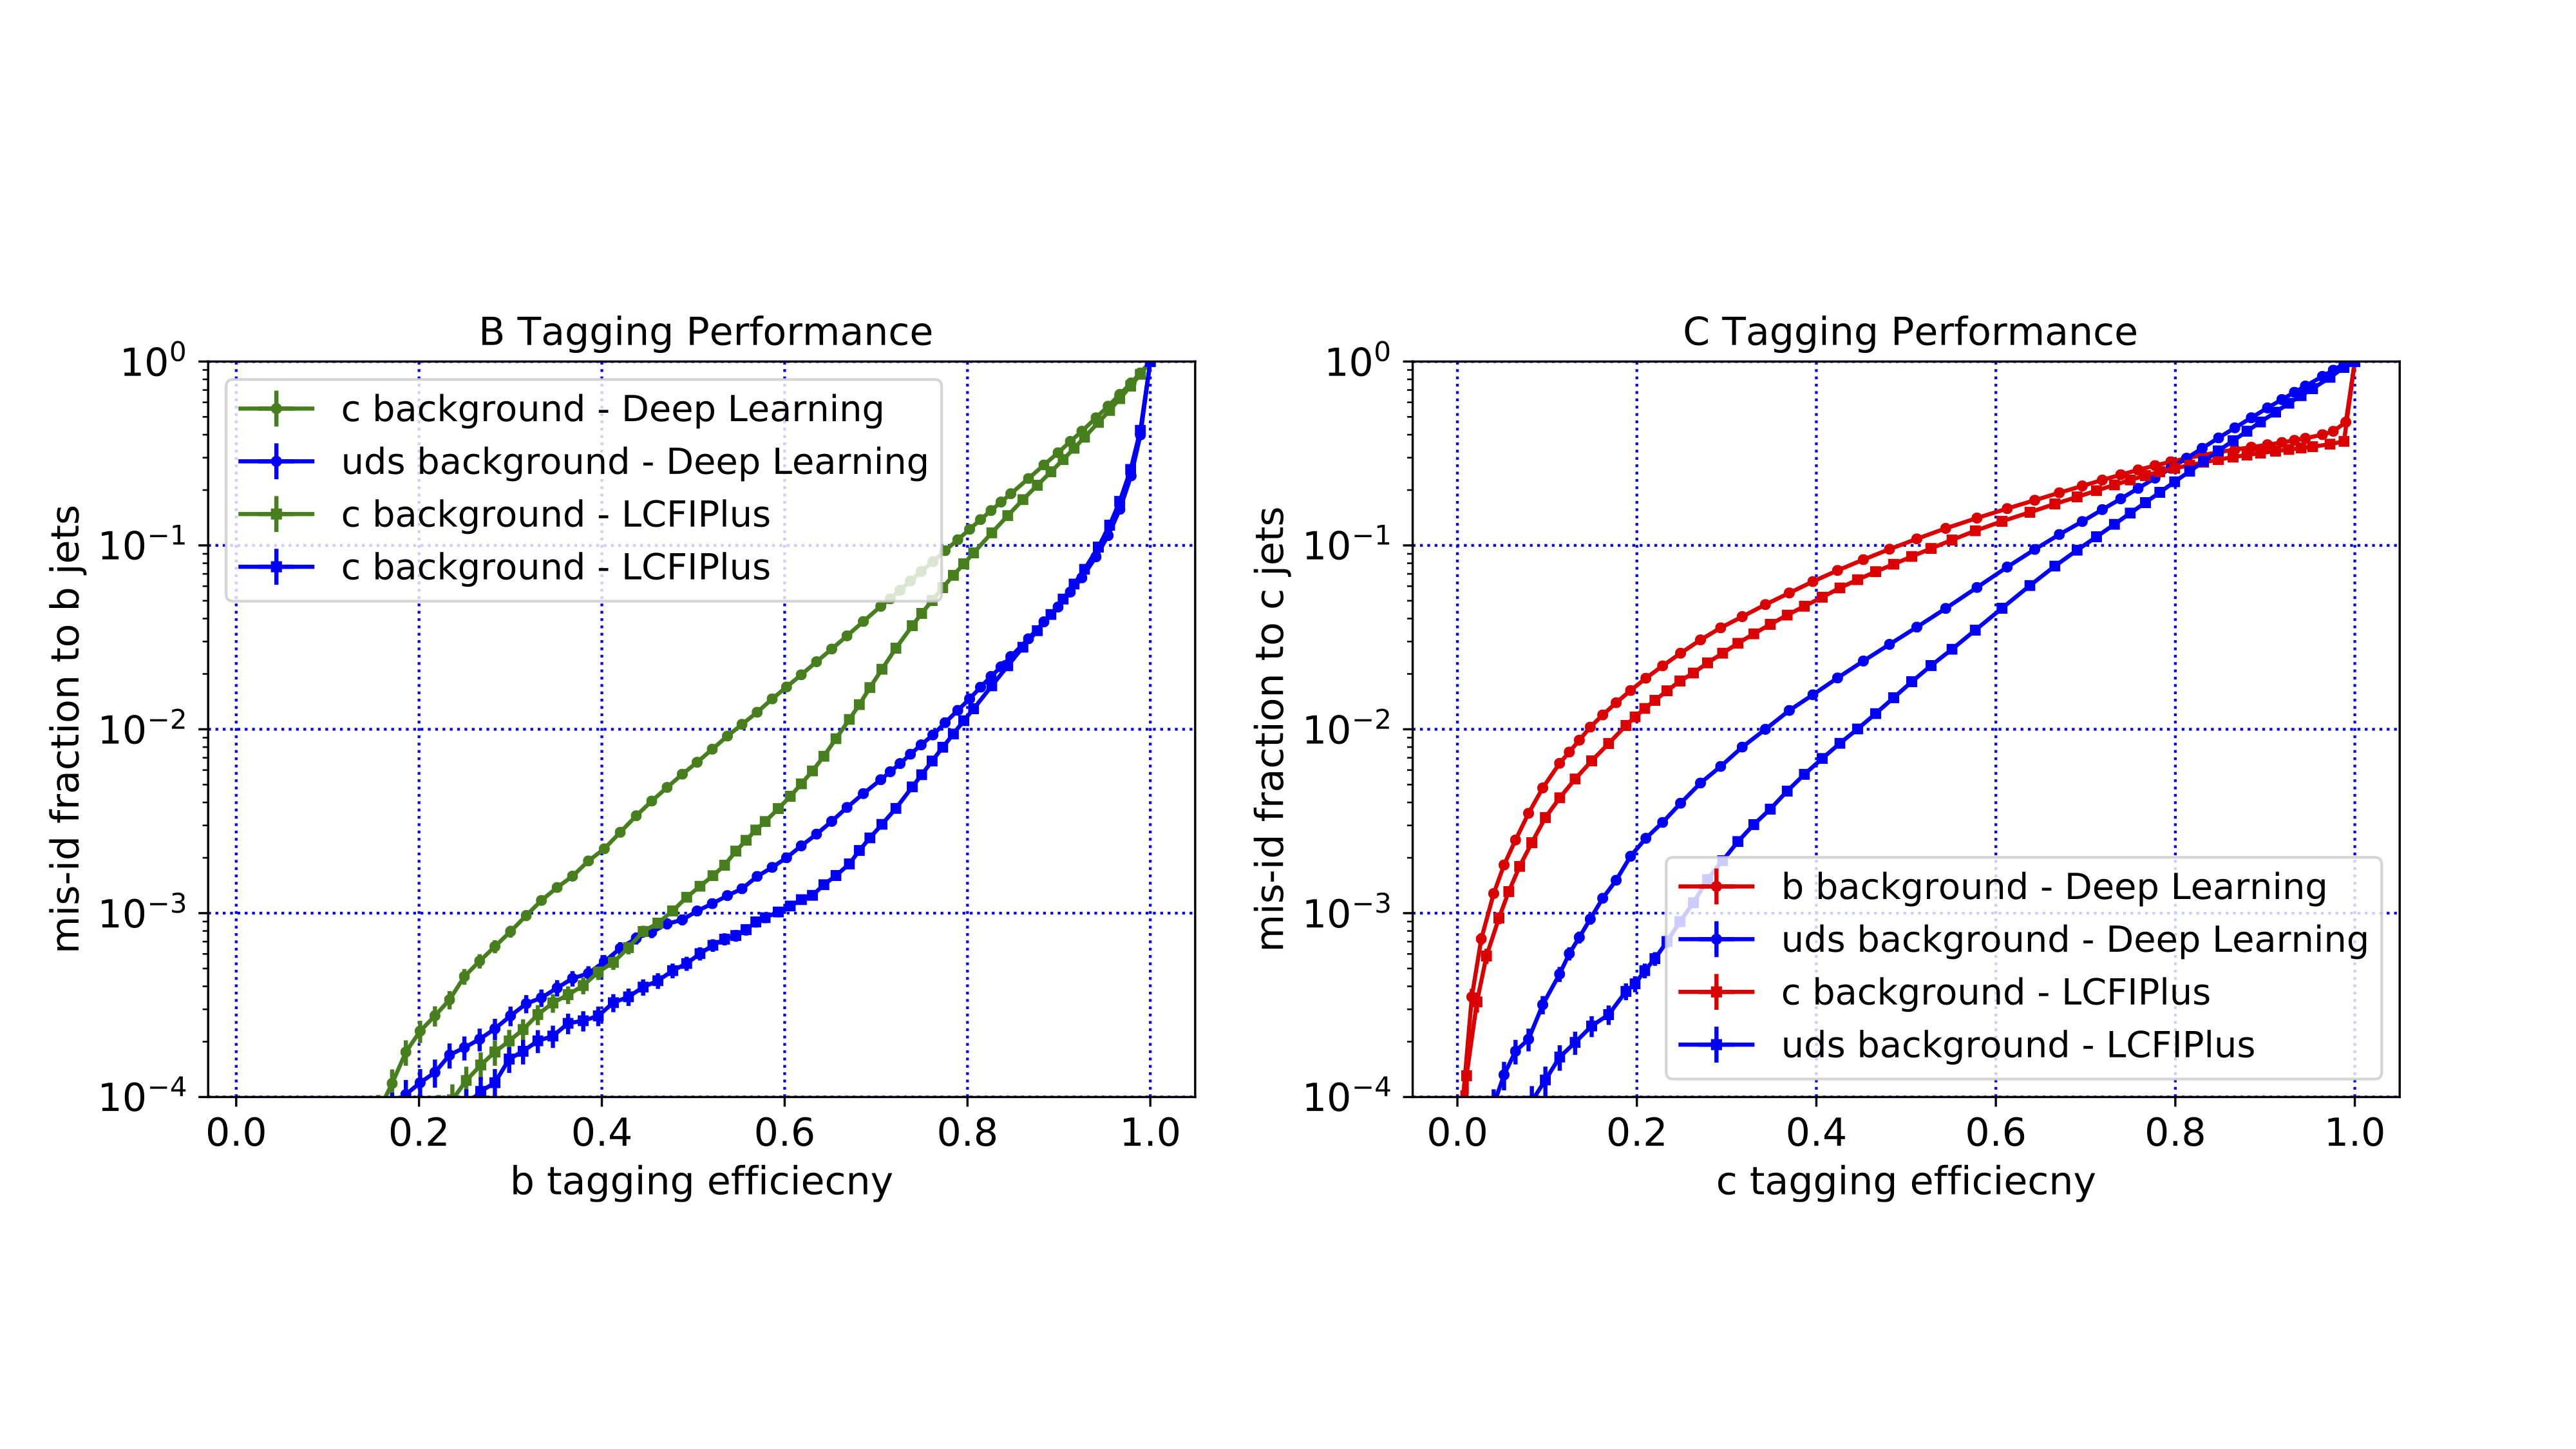
\includegraphics[width=1.0\textwidth, clip]{Figure/5Comparison/5-2-3-1FlavorTaggingROCCurve.png}
 \caption[フレーバータギングの性能に関するROC曲線]{フレーバータギングの性能に関するROC曲線}
 \label{5-2-3-1FlavorTaggingROCCurve}
\end{figure}























